\documentclass[aspectratio=169]{beamer}

% =====================================================
% RageFilter -- Apresentação de defesa (TCC2)
% Tema minimalista construído sobre o beamer padrão
% (sem dependências externas, compila com pdflatex puro)
% =====================================================

\usepackage[utf8]{inputenc}
\usepackage[T1]{fontenc}
\usepackage[brazil]{babel}
\usepackage{graphicx}
\usepackage{booktabs}
\usepackage{array}
\usepackage{xcolor}

\graphicspath{{figuras/}}

% ---------- Paleta minimalista ----------
\definecolor{primary}{HTML}{1B2631}   % grafite escuro
\definecolor{accent}{HTML}{C0392B}    % vermelho "rage"
\definecolor{secondary}{HTML}{7F8C8D} % cinza texto secundário
\definecolor{bgwhite}{HTML}{FFFFFF}

\renewcommand{\familydefault}{\sfdefault}

\setbeamertemplate{navigation symbols}{}
\setbeamercolor{background canvas}{bg=bgwhite}
\setbeamercolor{normal text}{fg=primary}
\setbeamercolor{frametitle}{fg=primary,bg=bgwhite}
\setbeamercolor{title}{fg=primary}
\setbeamercolor{itemize item}{fg=accent}
\setbeamercolor{itemize subitem}{fg=secondary}
\setbeamercolor{footline}{fg=secondary}
\setbeamercolor{page number in head/foot}{fg=secondary}
\setbeamertemplate{itemize item}{\textcolor{accent}{\textbullet}}
\setbeamertemplate{itemize subitem}{\textcolor{secondary}{--}}
\setbeamerfont{frametitle}{size=\Large,series=\bfseries}
\setbeamerfont{footline}{size=\tiny}

\setbeamertemplate{frametitle}{
  \vspace{0.3cm}
  \insertframetitle
  \vspace{0.15cm}
  {\color{accent}\rule{\textwidth}{0.6pt}}
}

\setbeamertemplate{footline}{
  \hbox{\begin{beamercolorbox}[wd=\paperwidth,ht=3ex,dp=1.2ex,right]{footline}
    \hspace*{1ex}RageFilter \hfill \insertframenumber{} / \inserttotalframenumber\hspace*{2ex}
  \end{beamercolorbox}}
}

\newcommand{\fonte}[1]{{\color{secondary}\tiny Fonte: #1}}

% ---------- Slide divisor de seção ----------
\newcommand{\sectiondivider}[2]{
  {
  \setbeamercolor{background canvas}{bg=primary}
  \begin{frame}[plain]
    \centering
    \vfill
    {\color{accent}\fontsize{60}{60}\selectfont\textbf{#1}}\\[0.4em]
    {\color{white}\Large #2}
    \vfill
  \end{frame}
  }
}

\title{RageFilter}
\author{Luiz Henrique Mendes de Oliveira Castro}
\date{2026}

\begin{document}

% ============== CAPA ==============
\begin{frame}[plain]
\centering
\vfill
{\color{primary}\Huge\textbf{RageFilter}}\\[0.5em]
{\Large Construção de um \textit{Dataset} de Toxicidade\\ para Comunidades \textit{Gamer} Brasileiras}\\[1.2em]
{\color{accent}\rule{4cm}{1pt}}\\[1.2em]
{\large Luiz Henrique Mendes de Oliveira Castro}\\[0.3em]
{\small\color{secondary} Orientador: Marcelo Arêas Rodrigues da Silva, D.Sc.}\\[0.6em]
{\small\color{secondary} CEFET/RJ --- 2026}
\vfill
\end{frame}

% ============== AGENDA ==============
\begin{frame}{Sumário}
\begin{itemize}
    \item \textcolor{accent}{\textbf{1.}} Introdução
    \item \textcolor{accent}{\textbf{2.}} Fundamentação Teórica e Trabalhos Relacionados
    \item \textcolor{accent}{\textbf{3.}} Desenvolvimento e Caracterização do \textit{Dataset}
    \item \textcolor{accent}{\textbf{4.}} Conclusão
\end{itemize}
\end{frame}

% =====================================================
\sectiondivider{1}{Introdução}
% =====================================================

\begin{frame}{Contexto}
\begin{itemize}
    \item Jogos digitais $\rightarrow$ grandes espaços de socialização (Twitch, Reddit, Discord)
    \item Crescimento acompanhado de \textbf{comportamento tóxico}: agressão, assédio, discurso de ódio
    \item IA + PLN como ferramentas de moderação automatizada
    \item \textbf{Lacuna:} poucos \textit{datasets} em português voltados ao vocabulário \textit{gamer}
\end{itemize}
\end{frame}

\begin{frame}{Problema}
\begin{center}
\Large
Como construir um \textit{dataset} especializado capaz de representar a toxicidade textual em comunidades \textit{gamer} brasileiras, considerando suas particularidades linguísticas?
\end{center}
\end{frame}

\begin{frame}{Objetivos}
\textbf{Geral:} construir um \textit{dataset} de toxicidade para comunidades \textit{gamer} brasileiras, com mensagens rotuladas e taxonomia de termos ofensivos.

\vspace{0.3cm}
\textbf{Específicos:}
\begin{itemize}
    \item Coletar mensagens de plataformas \textit{gamer} (Twitch)
    \item Definir taxonomia de toxicidade adequada ao contexto
    \item Construir léxico de gírias e termos ofensivos
    \item Limpar, padronizar e rotular as mensagens
    \item Disponibilizar o recurso para pesquisas futuras
\end{itemize}
\end{frame}

% =====================================================
\sectiondivider{2}{Fundamentação Teórica e\\Trabalhos Relacionados}
% =====================================================

\begin{frame}{Toxicidade em Jogos \textit{Online}}
\begin{columns}
\column{0.5\textwidth}
\begin{itemize}
    \item Insultos de habilidade (\textit{"noob"}, "lixo")
    \item Discriminação, ameaças, assédio
    \item Anonimato + competitividade $\rightarrow$ normalização
\end{itemize}
\column{0.5\textwidth}
\centering
{\color{accent}\Huge\textbf{90\%}}\\{\small já testemunharam toxicidade}\\[0.5em]
{\color{accent}\Huge\textbf{40\%}}\\{\small admitem já ter sido tóxicos}
\end{columns}
\vspace{0.3cm}
\fonte{Pires e Fortim (2024); Nunes e Fortim (2025)}
\end{frame}

\begin{frame}{Modelos de PLN para Detecção de Toxicidade}
\begin{itemize}
    \item Transformers: BERT, RoBERTa, \textbf{BERTimbau}, BERTweet.BR
    \item GameTox: \textit{intent classification} + \textit{slot filling} (token a token)
    \item BERTimbau + propagação semi-supervisionada $\rightarrow$ competitivo com poucos dados rotulados
    \item Risco: modelos generalistas (Detoxify, Perspective API) dependem demais de palavras-chave isoladas, ignorando contexto
\end{itemize}
\end{frame}

\begin{frame}{Taxonomia Adotada -- Nível de Sentença}
\small
\begin{tabular}{>{\bfseries}p{2.3cm}p{8.7cm}}
\toprule
NT & Não tóxico \\
INS & Insulto (habilidade, desempenho, identidade) \\
ASS & Assédio direcionado e persistente \\
DO & Discurso de ódio (raça, gênero, orientação, religião) \\
AME & Ameaça de violência \\
OBS & Obscenidade / palavrão genérico \\
\bottomrule
\end{tabular}
\vspace{0.3cm}

\centering\textit{+ nível de \textit{token} (\textit{slot filling}):} \textbf{TÓXICO} \textbar{} \textbf{GÍRIA\_GAMER} \textbar{} \textbf{NEUTRO}
\end{frame}

\begin{frame}{Trabalhos Relacionados -- Destaques}
\begin{itemize}
    \item \textbf{GameTox} (Naseem et al., 2025) -- 53 mil msgs, \textit{World of Tanks}, inglês, anotação manual
    \item \textbf{ToLD-BR / BERTimbau} (Ricarte Neto et al., 2025) -- toxicidade em PT-BR com poucos dados rotulados
    \item \textbf{Cascatas de toxicidade na Twitch} (Lobo, Barbosa e Melo, 2025) -- PT-BR, mesma plataforma deste trabalho
    \item \textbf{SHAP + Detoxify} (Melo e Figueredo, 2025) -- modelos dependem de palavras-chave isoladas
    \item \textbf{Comparação de 6 \textit{datasets}} (Fortuna et al., 2020) -- inconsistência entre taxonomias
\end{itemize}
\end{frame}

% =====================================================
\sectiondivider{3}{Desenvolvimento e\\Caracterização do \textit{Dataset}}
% =====================================================

\begin{frame}{Arquitetura da Solução}
\centering
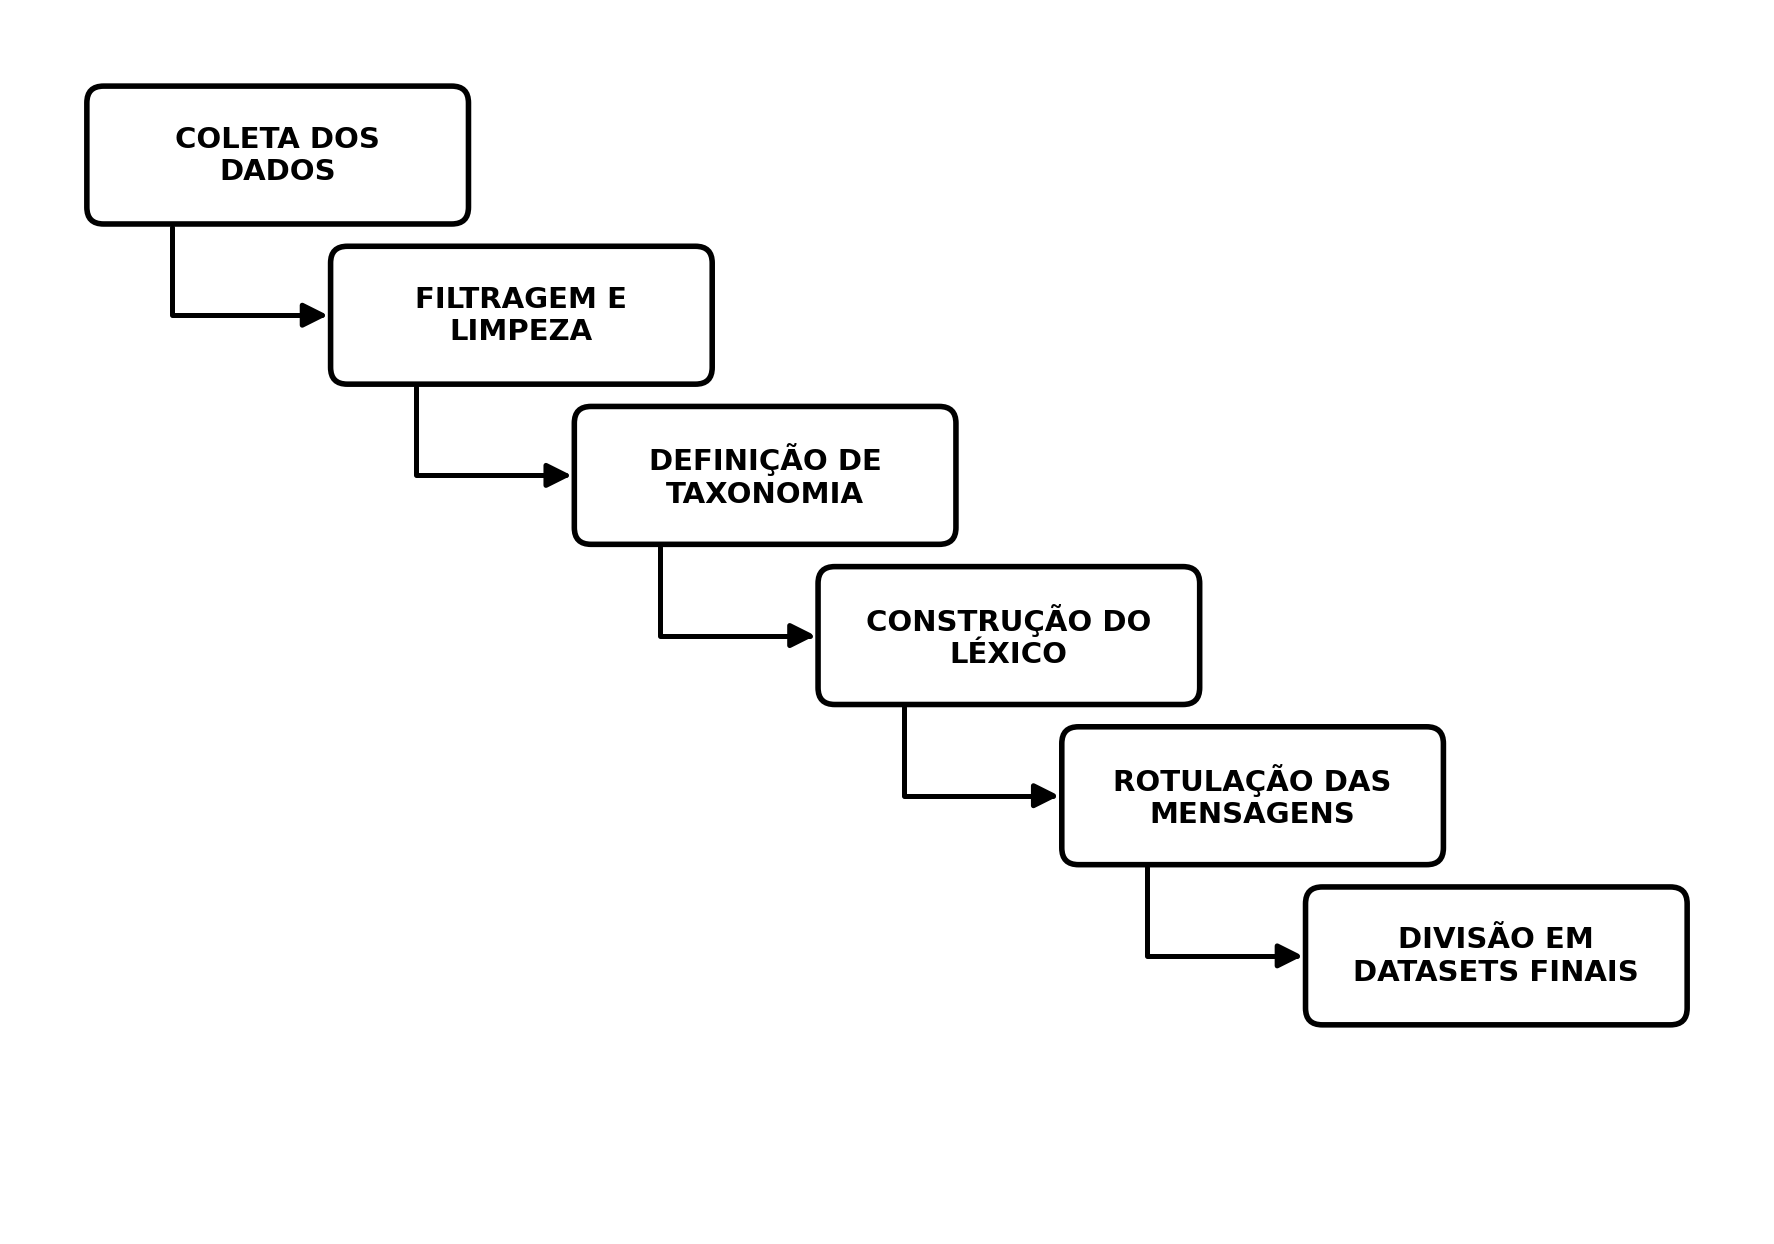
\includegraphics[width=0.78\textwidth]{fig_arquitetura.png}
\end{frame}

\begin{frame}{Coleta de Dados}
\begin{itemize}
    \item \textit{Scraper} em Node.js (\texttt{tmi.js}) -- chat ao vivo da Twitch
    \item \textbf{49 canais} configurados, \textbf{30 ativos} durante a coleta
    \item Período: \textbf{abril -- junho de 2026}
    \item Perfis: League of Legends, CS2/FPS, \textit{streamers} de variedade
    \item Apenas mensagens \textbf{públicas} de chat
\end{itemize}
\end{frame}

\begin{frame}{Pipeline de Limpeza}
\centering
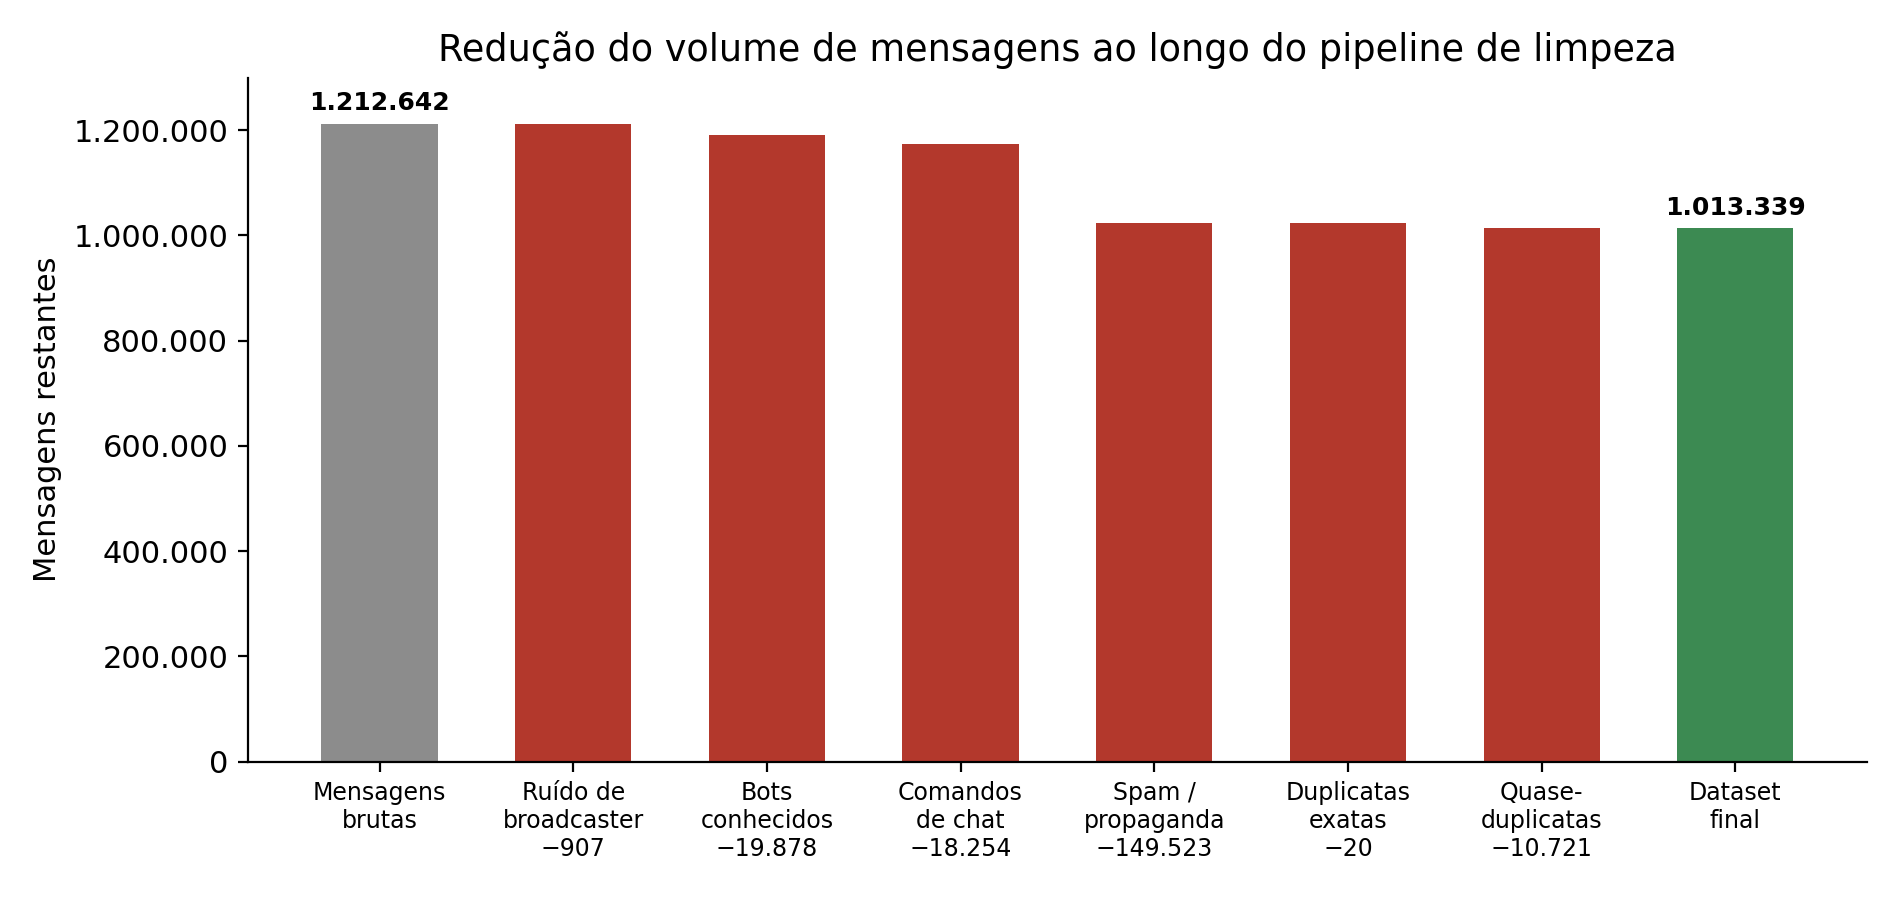
\includegraphics[width=0.95\textwidth]{fig_pipeline_limpeza.png}
\vspace{0.2cm}\\
{\small \textbf{1,2 milhão} de mensagens brutas $\rightarrow$ \textbf{1.013.339} mensagens finais}
\end{frame}

\begin{frame}{Léxico e Rotulação Automática}
\begin{itemize}
    \item \texttt{lexicon.csv}: \textbf{500+ termos} (gírias, insultos, ódio, obscenidade, ameaça)
    \item Variações morfológicas e \textit{leetspeak} (\textit{m4c4c0})
    \item Termos ambíguos (\textit{noob}, \textit{bot}, \textit{hacker}) só ofendem com direcionamento (@usuário)
    \item Ameaça $\rightarrow$ padrões de frase (regex)
    \item Assédio $\rightarrow$ heurística: mesmo remetente, mesmo alvo, $\geq$3x em 5 min
    \item Sem uso de LLM nem anotação manual nesta etapa
\end{itemize}
\end{frame}

\begin{frame}{Distribuição dos Rótulos -- Sentença}
\centering
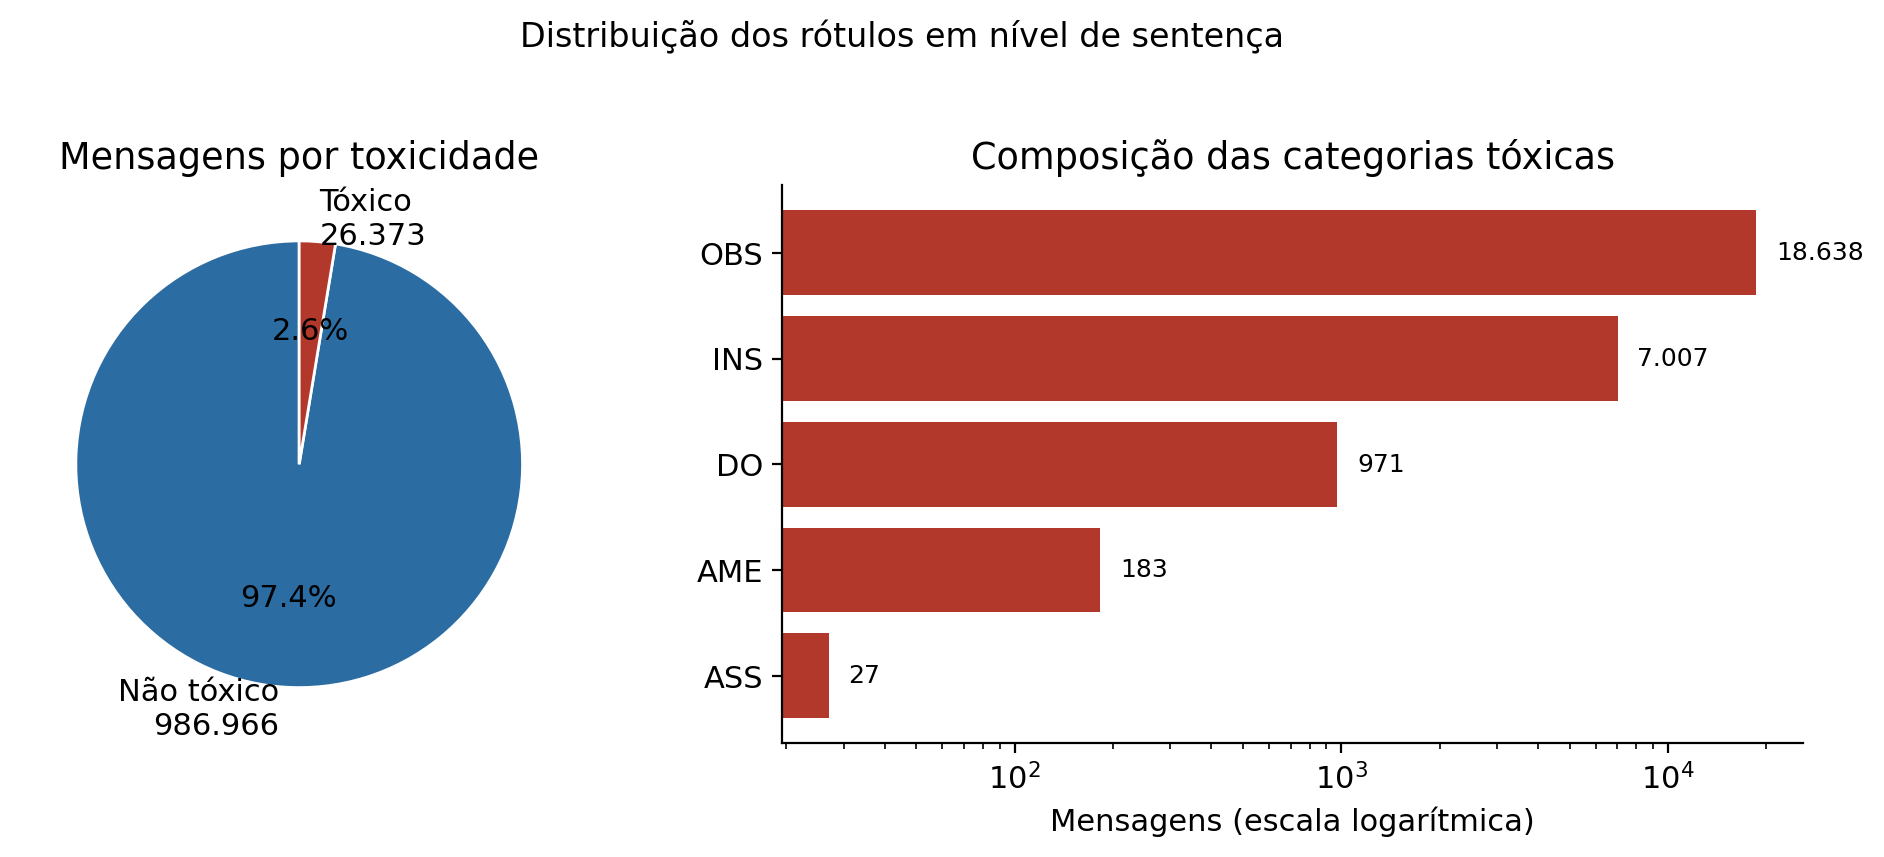
\includegraphics[width=0.7\textwidth]{fig_distribuicao_sentenca.png}
\vspace{0.2cm}\\
{\small \textbf{2,60\%} das mensagens são tóxicas (97,40\% NT)}
\end{frame}

\begin{frame}{Distribuição dos Rótulos -- Token}
\centering
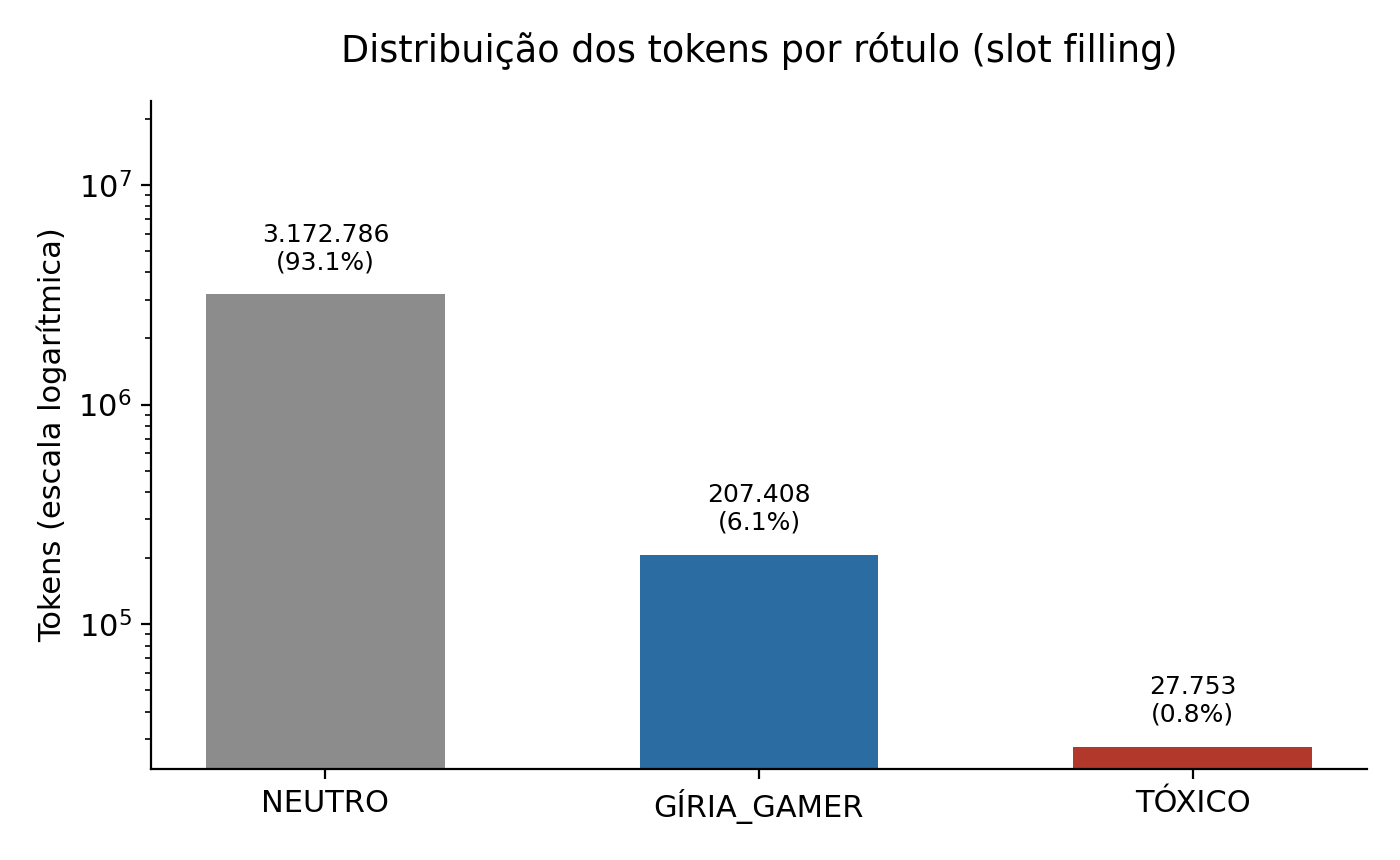
\includegraphics[width=0.55\textwidth]{fig_distribuicao_token.png}
\vspace{0.2cm}\\
{\small NEUTRO 93,1\% \quad GÍRIA\_GAMER 6,1\% \quad TÓXICO 0,8\%}
\end{frame}

\begin{frame}{Toxicidade por Canal}
\centering
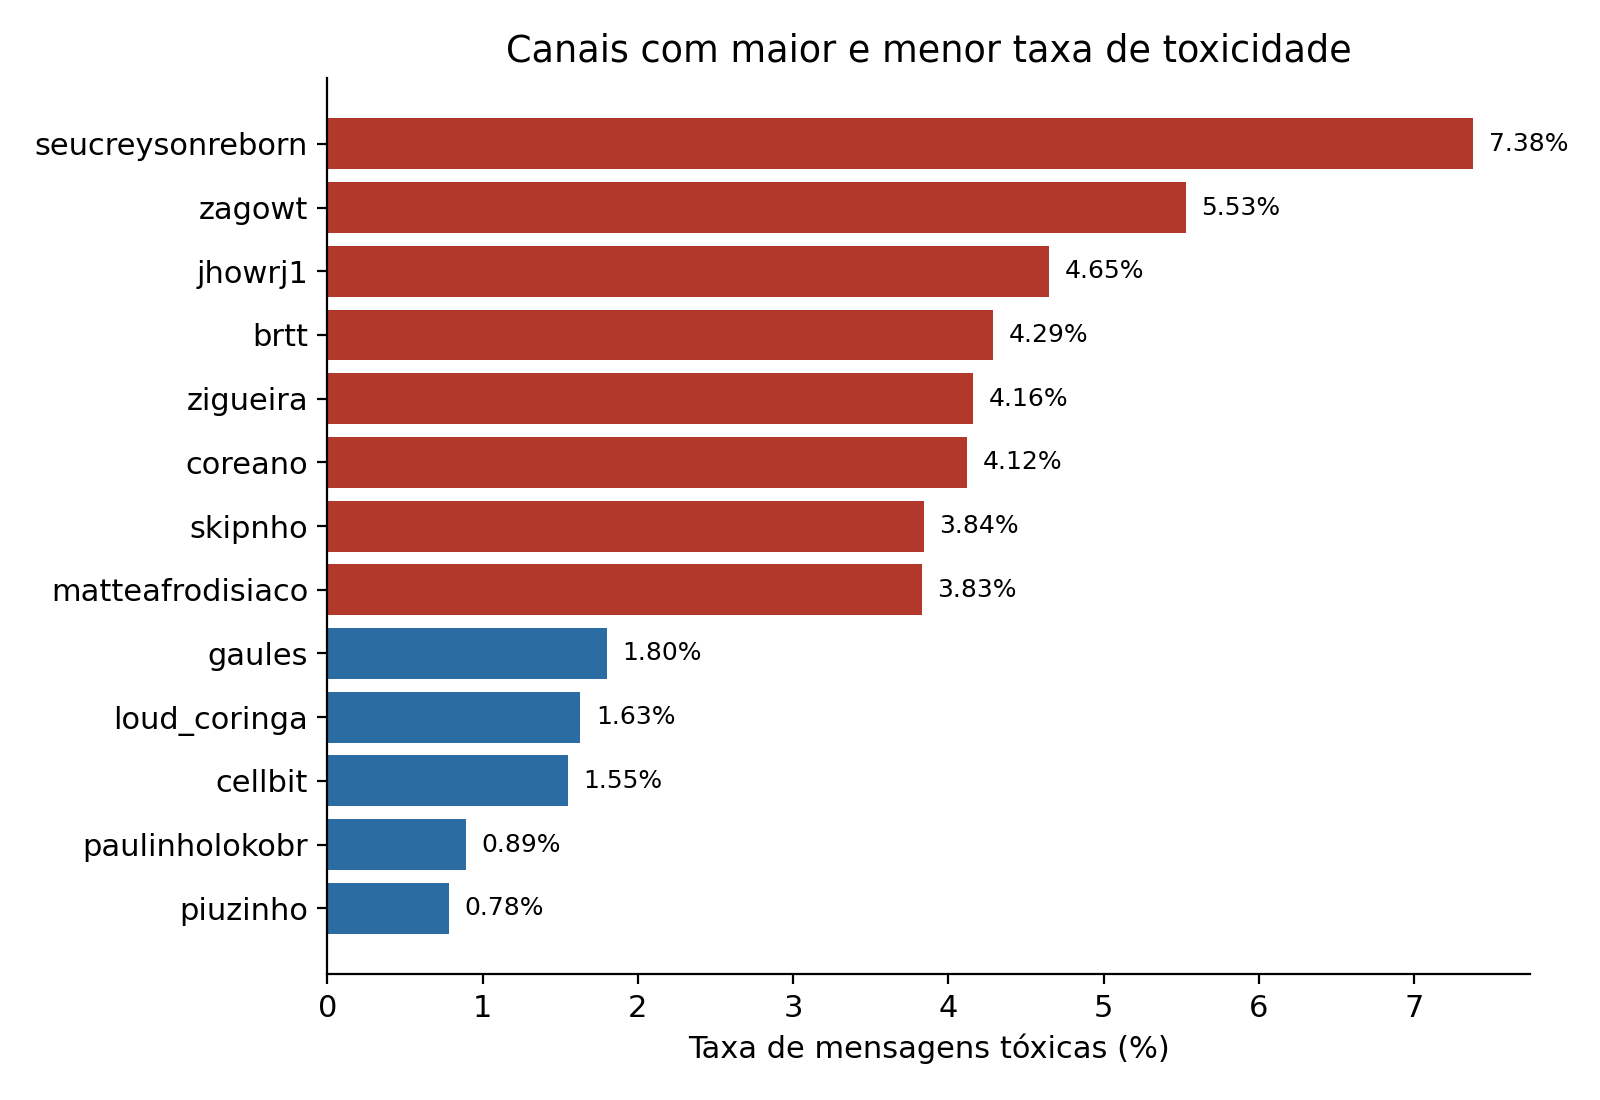
\includegraphics[width=0.85\textwidth]{fig_ranking_canais.png}
\vspace{0.2cm}\\
{\small Variação de menos de 1\% a mais de 7\% entre canais}
\end{frame}

\begin{frame}{Nuvens de Palavras}
\centering
\begin{minipage}{0.31\textwidth}
\centering
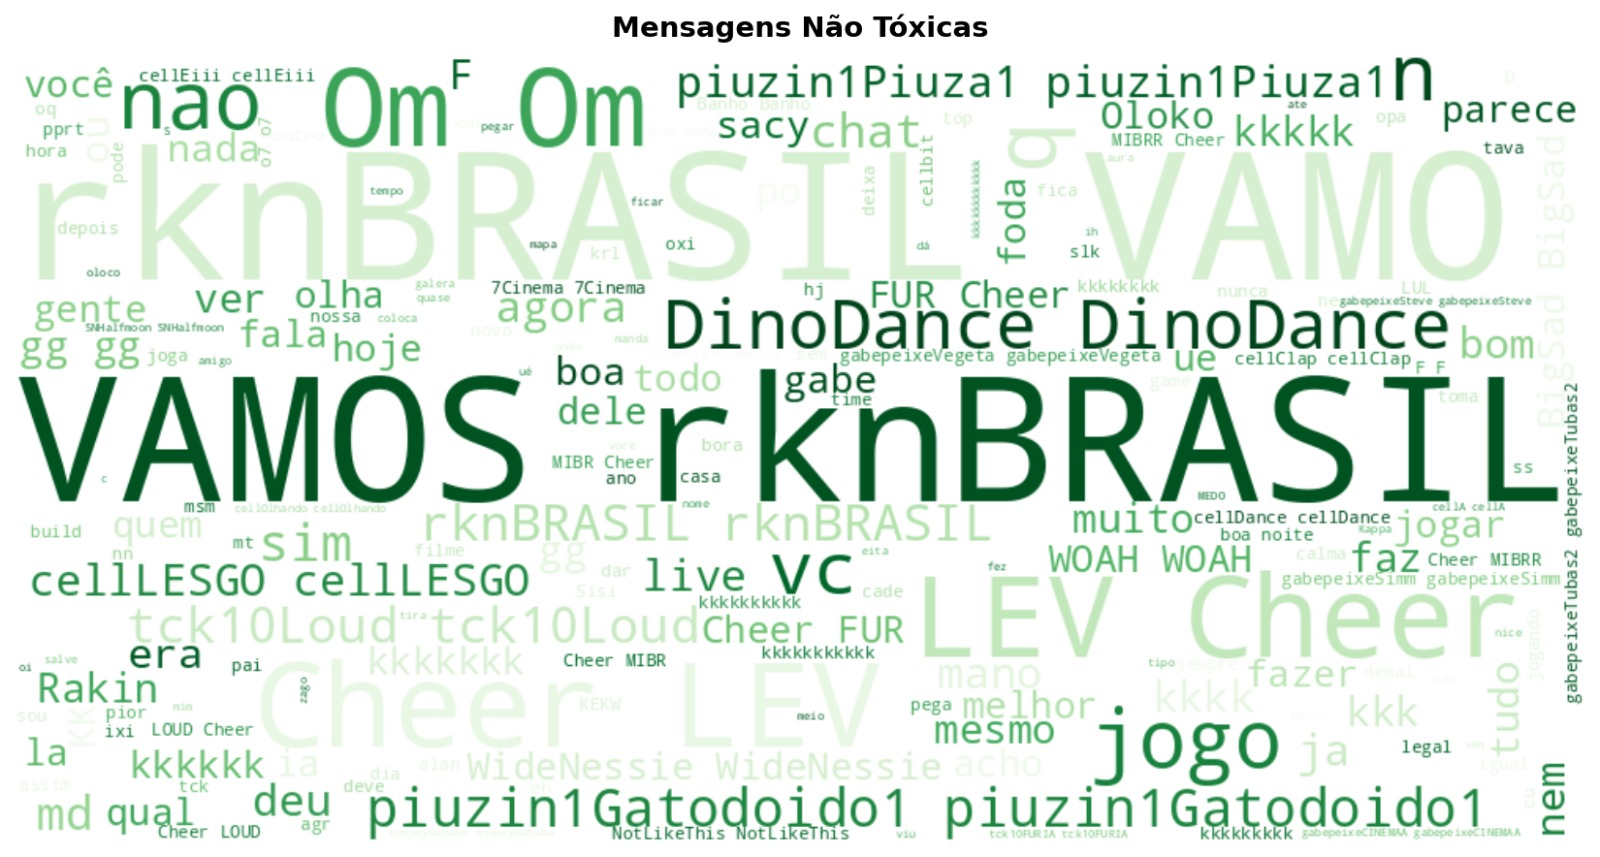
\includegraphics[width=\textwidth]{fig_nuvem_neutras.jpeg}\\
{\tiny Não tóxicas}
\end{minipage}\hfill
\begin{minipage}{0.31\textwidth}
\centering
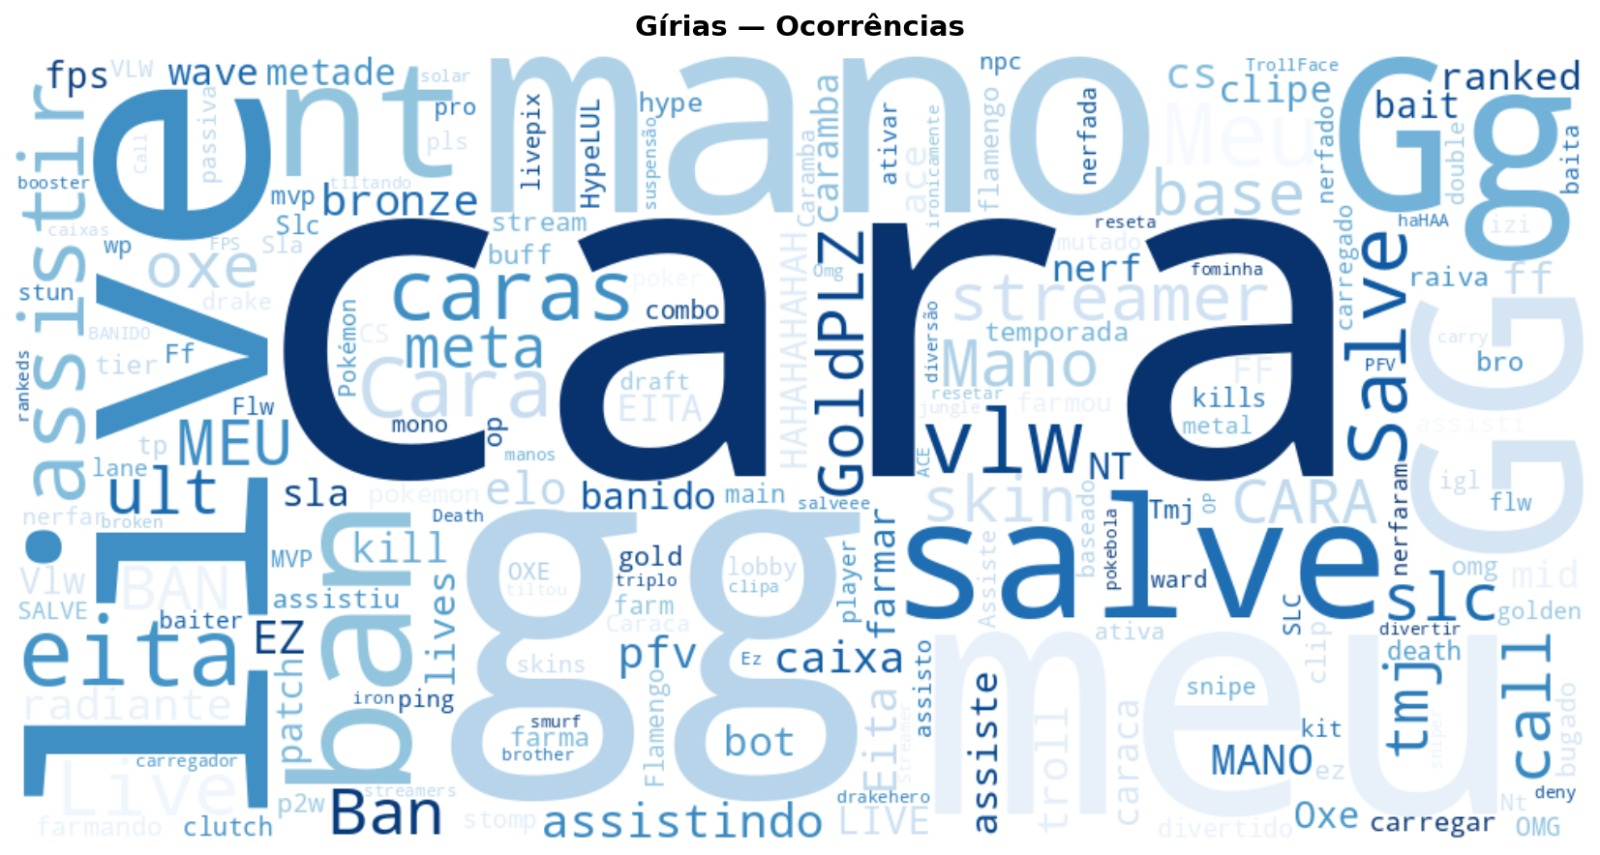
\includegraphics[width=\textwidth]{fig_nuvem_girias.jpeg}\\
{\tiny Gírias \textit{gamer}}
\end{minipage}\hfill
\begin{minipage}{0.31\textwidth}
\centering
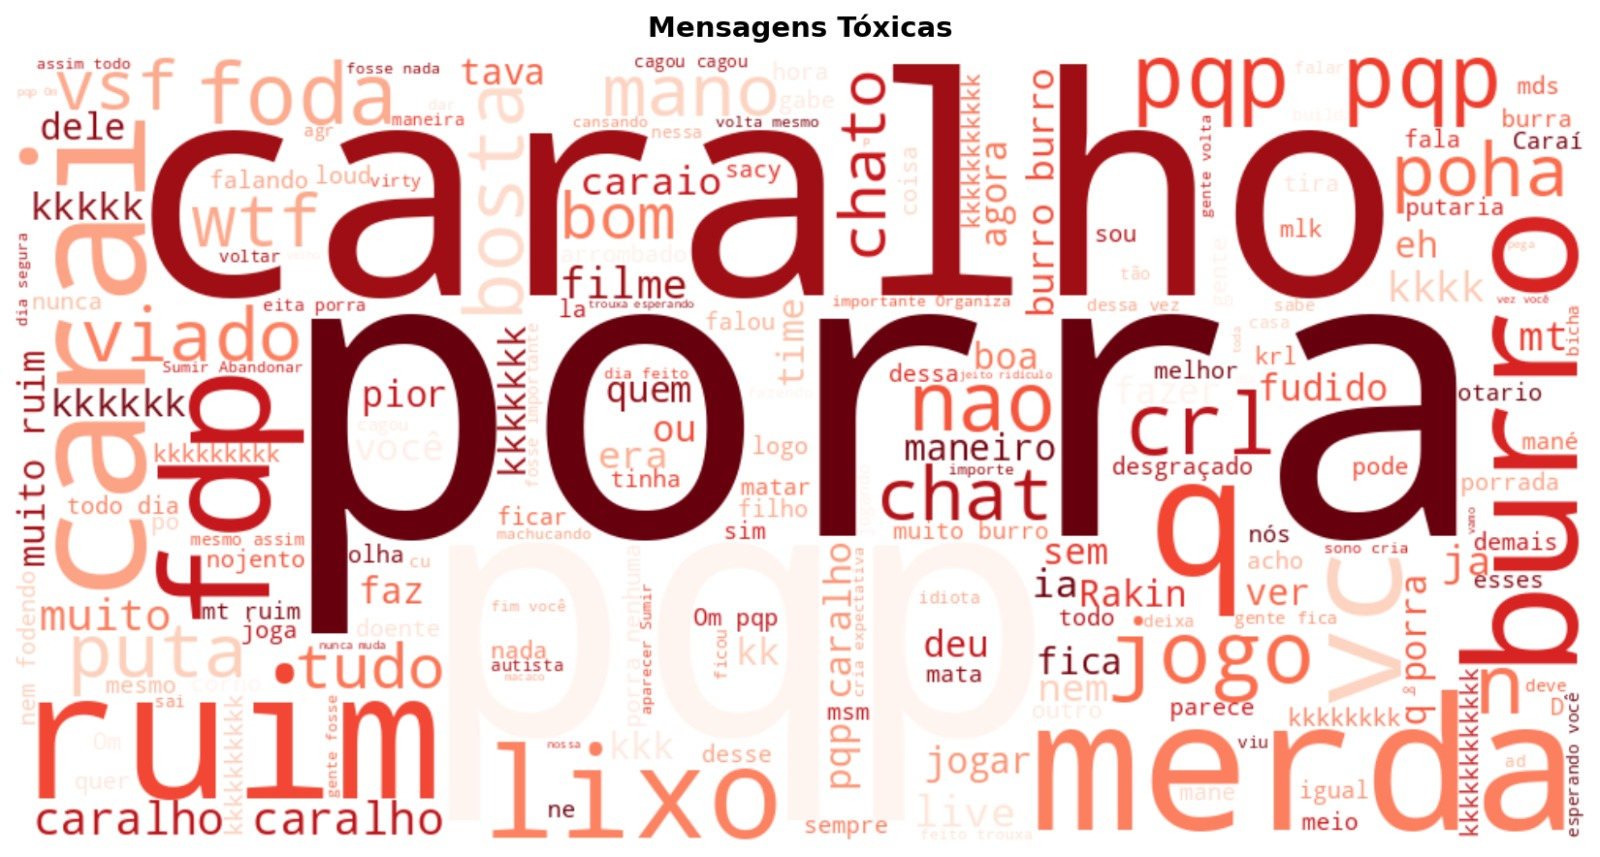
\includegraphics[width=\textwidth]{fig_nuvem_toxicas.jpeg}\\
{\tiny Tóxicas}
\end{minipage}
\end{frame}

\begin{frame}{Dataset Final em Números}
\centering
\begin{columns}
\column{0.33\textwidth}
\centering{\color{accent}\Huge\textbf{1,01M}}\\{\small mensagens}
\column{0.33\textwidth}
\centering{\color{accent}\Huge\textbf{30}}\\{\small canais}
\column{0.33\textwidth}
\centering{\color{accent}\Huge\textbf{500+}}\\{\small termos no léxico}
\end{columns}
\vspace{0.6cm}
{\small vs. GameTox: 53 mil mensagens, 1 jogo, inglês, anotação manual}\\
{\footnotesize\color{secondary} Vantagem de escala e especialização linguística -- não de rigor de anotação}
\end{frame}

% =====================================================
\sectiondivider{4}{Conclusão}
% =====================================================

\begin{frame}{Contribuições}
\begin{itemize}
    \item \textit{Dataset} de \textbf{+1 milhão} de mensagens em PT-BR do universo \textit{gamer}
    \item Rotulado em \textbf{dois níveis}: sentença (6 categorias) e \textit{token} (\textit{slot filling})
    \item Léxico reutilizável de gírias e termos ofensivos \textit{gamer}
    \item \textit{Pipeline} completo: coleta $\rightarrow$ limpeza $\rightarrow$ rotulação $\rightarrow$ exportações
\end{itemize}
\end{frame}

\begin{frame}{Limitações}
\begin{itemize}
    \item Rotulação por \textbf{léxico/regras}, não por anotação humana
    \item Heurísticas não captam sarcasmo, brincadeira ou contexto implícito
    \item Obscenidade coloquial nem sempre indica toxicidade real
    \item Corpus concentrado em poucos canais de grande audiência
    \item Coleta restrita à Twitch (sem Reddit/Discord)
    \item Anonimização de usuários ainda pendente
\end{itemize}
\end{frame}

\begin{frame}{Trabalhos Futuros}
\begin{itemize}
    \item Concluir validação humana da amostra estratificada (protocolo já definido)
    \item Expandir o léxico (gírias regionais, novos jogos)
    \item Treinar classificadores \textit{transformer} (BERTimbau, mBERT) sobre o \textit{dataset} rotulado
\end{itemize}
\end{frame}

{
\setbeamercolor{background canvas}{bg=primary}
\begin{frame}[plain]
\centering
\vfill
{\color{white}\Huge\textbf{Obrigado}}\\[0.5em]
{\color{accent}\Large Perguntas?}
\vfill
\end{frame}
}

\end{document}
